% --------------------------------------------------- %
%						Capa						  %
% --------------------------------------------------- %
% >>> Capa Personalizada
\renewcommand{\imprimircapa}{%
	\begin{capa}%
		\center
		{\ABNTEXchapterfont\bfseries\large\imprimirINSTITUICAO}
			\vspace*{1.5cm}
		\includegraphics*[width=0.25\textwidth]{brasao_ufes.jpg}
			\vspace*{1.5cm} \\
		{\ABNTEXchapterfont\bfseries\Large\MakeUppercase\imprimirautor}
				\vspace*{2.5cm} \\
		{\ABNTEXchapterfont\bfseries\Large\imprimirtitulo}
			\vfill
			\vspace*{0.5cm}
		{\large\MakeUppercase\imprimirlocal}
		\par
		{\large\MakeUppercase\imprimirdata}
			\vspace*{1cm}
	\end{capa}
}

\imprimircapa

% --------------------------------------------------- %
%					Folha de Rosto 					  %
% --------------------------------------------------- %
% >> O * indica que haverá a ficha bibliográfica

\renewcommand{\imprimirfolhaderosto}{

\begin{folhaderosto}
	\begin{center}
    	{\ABNTEXchapterfont\large\imprimirautor}
		    \vspace*{\fill}\vspace*{\fill}
    	\begin{center}
	    	\ABNTEXchapterfont\bfseries\Large\imprimirtitulo
	    \end{center}
    		\vspace*{\fill}
    		\hspace{.45\textwidth}
	    \begin{minipage}{.5\textwidth}
        	\imprimirpreambulo
	    \end{minipage}
    		\vspace*{\fill}
	    \end{center}  
        \begin{center}
        	% >> Se necessáiro, ajustar os \vspace
        	%\vspace*{0.5cm}
        {\large\imprimirlocal}
        \par
        {\large\imprimirdata}
       		%\vspace*{1cm}
      \end{center}
\end{folhaderosto}
}

\imprimirfolhaderosto

% --------------------------------------------------- %
%					Ficha Catalográfica 			  %
% --------------------------------------------------- %

% Isto é um exemplo de Ficha Catalográfica, ou ``Dados internacionais de
% catalogação-na-publicação''. Você pode utilizar este modelo como referência. 
% Porém, provavelmente a biblioteca da sua universidade lhe fornecerá um PDF
% com a ficha catalográfica definitiva após a defesa do trabalho. Quando estiver
% com o documento, salve-o como PDF no diretório do seu projeto e substitua todo
% o conteúdo de implementação deste arquivo pelo comando abaixo:
%
% \begin{fichacatalografica}
%     \includepdf{fig_ficha_catalografica.pdf}
% \end{fichacatalografica}

%\begin{fichacatalografica}
%	\sffamily
%	\vspace*{\fill}					% Posição vertical
%	\begin{center}					% Minipage Centralizado
%	\fbox{\begin{minipage}[c][8cm]{13.5cm}		% Largura
%	\small
%	\imprimirautor
%	%Sobrenome, Nome do autor
%	
%	\hspace{0.5cm} \imprimirtitulo  / \imprimirautor. --
%	\imprimirlocal, \imprimirdata-
%	
%	\hspace{0.5cm} \pageref{LastPage} p. : il. (algumas color.) ; 30 cm.\\
%	
%	\hspace{0.5cm} \imprimirorientadorRotulo~\imprimirorientador\\
%	
%	\hspace{0.5cm}
%	\parbox[t]{\textwidth}{\imprimirtipotrabalho~--~\imprimirinstituicao,
%	\imprimirdata.}\\
%	
%	\hspace{0.5cm}
%		1. Palavra-chave1.
%		2. Palavra-chave2.
%		2. Palavra-chave3.
%		I. Orientador.
%		II. Universidade xxx.
%		III. Faculdade de xxx.
%		IV. Título 			
%	\end{minipage}}
%	\end{center}
%\end{fichacatalografica}

% --------------------------------------------------- %
%					Folha de Aprovação			      %
% --------------------------------------------------- %
% >>> Após apresentação do trabalho, substitua todo o conteúdo 
% por uma imagem da página assinada pela banca com o comando abaixo:
\ifisFolhaAprovacao
%TCC finalizado
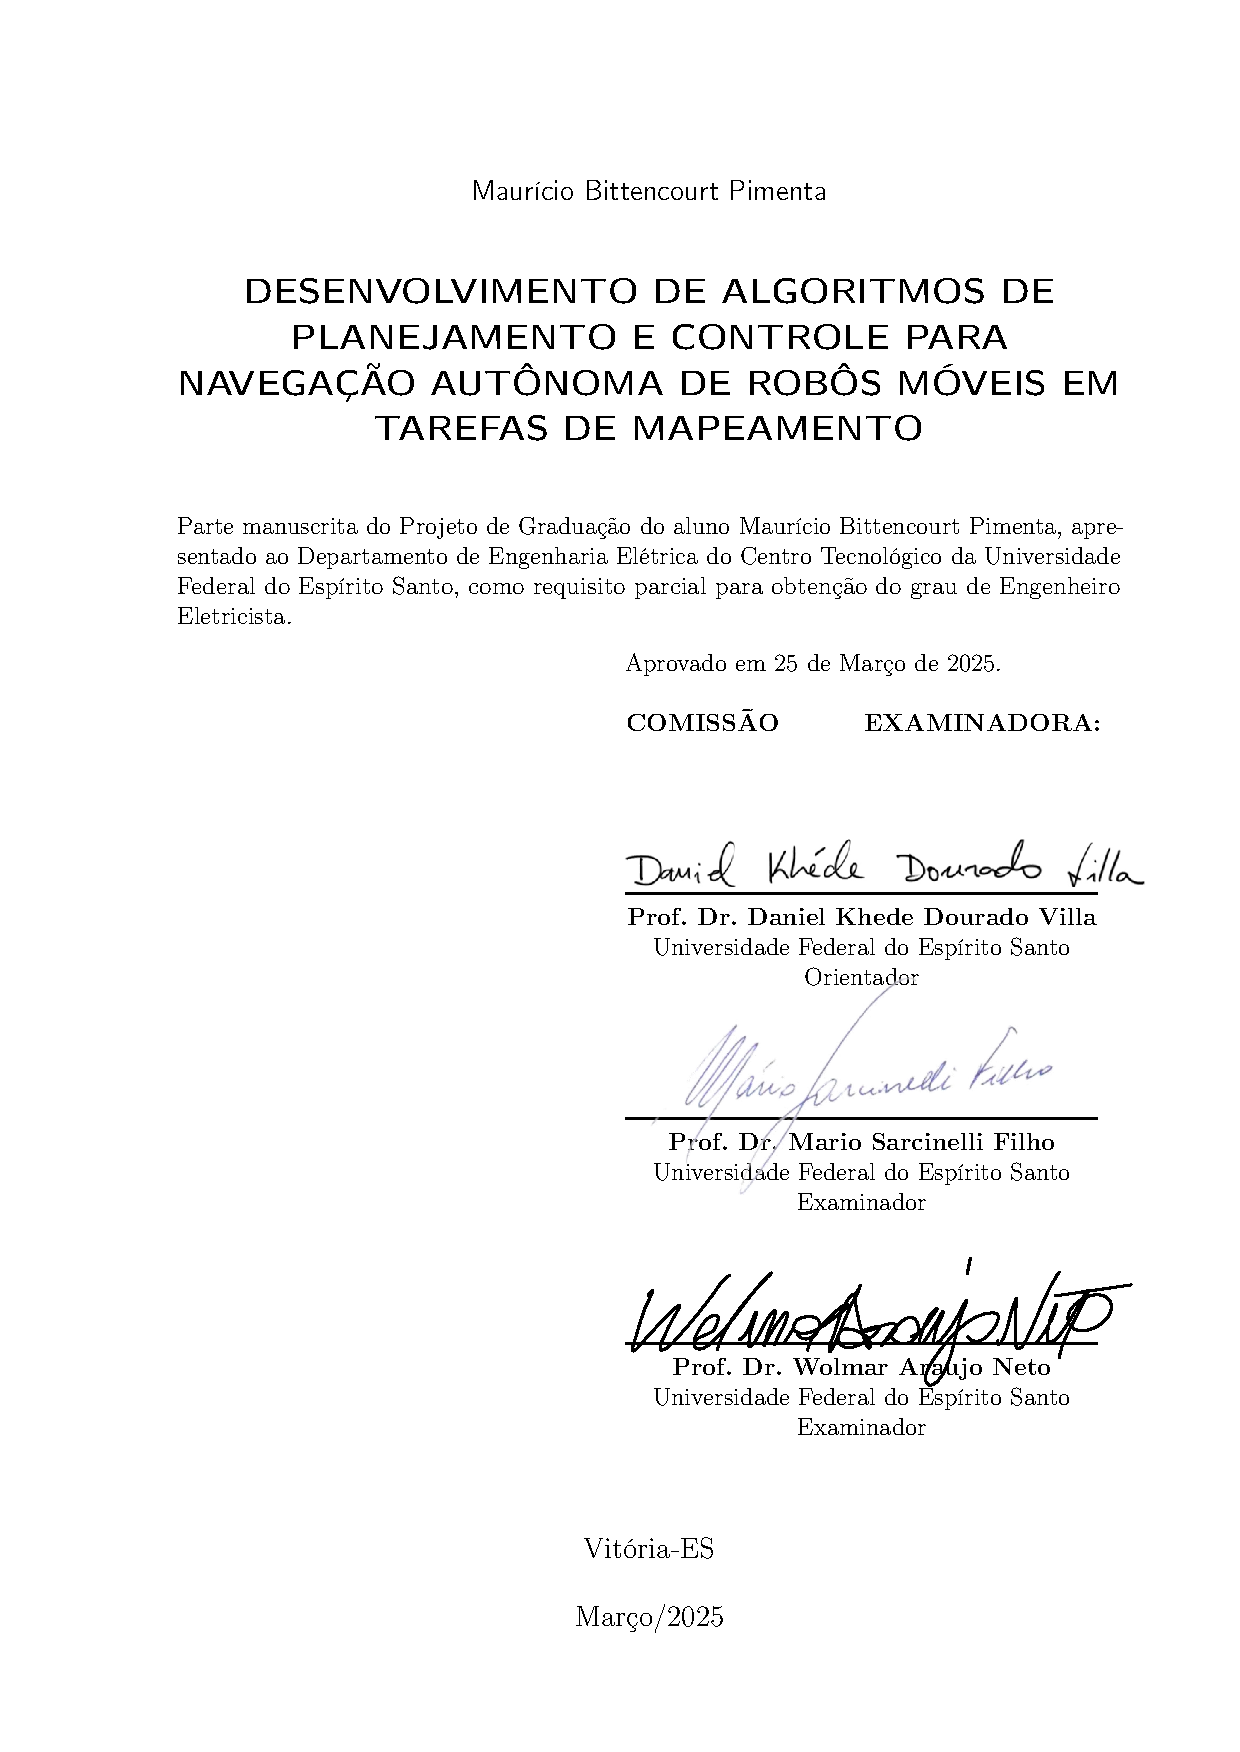
\includepdf{aprovacao.pdf}
\else
%TCC não finalizado
\begin{folhadeaprovacao}
   \begin{center}
     {\ABNTEXchapterfont\large\imprimirautor}
 	\begin{center}
      	\ABNTEXchapterfont\bfseries\Large\imprimirtitulo
     \end{center}
     %\vspace*{\fill}
   \end{center}    
     \imprimirpreambulo
 		\vspace{-0.5cm}
     \begin{center}
 		\hspace{.45\textwidth}
     \begin{minipage}{.5\textwidth}
         Aprovado em x de xxxx de 20xx. \\\\
         \textbf{COMISSÃO EXAMINADORA:}
         \vspace{0.5cm}
         \assinatura{\textbf{\imprimirorientador} \\ Universidade Federal do Espírito Santo \\ Orientador}
         %\vspace{1.0cm}
%        \assinatura{\textbf{\imprimircoorientador} \\ Universidade Federal do Espírito Santo \\ Coorientadora}
        \vspace{1.0cm}
 		\assinatura{\textbf{Prof. Dr. XXXXX} \\ Universidade Federal do Espírito Santo \\ Examinador}
 		\vspace{1.0cm}
 		\assinatura{\textbf{Prof. Msc. YYYYY} \\ Universidade Federal do Espírito Santo \\ Examinador}
     \end{minipage}
 	    \vspace*{\fill}
    \end{center}
         
    \begin{center}
       	% >> Se necessáiro, ajustar os \vspace
 		%\vspace*{0.5cm}
     	{\large\imprimirlocal}
     	\par
     	{\large\imprimirdata}
    		%\vspace*{1cm}
   \end{center}  
 \end{folhadeaprovacao}
\fi
% --------------------------------------------------- %
%						Dedicatória				      %
% --------------------------------------------------- %
\begin{dedicatoria}
   \vspace*{\fill}
   \centering
   \noindent
   \textit{Quem agradeceria a alguém por inventar o Python? Vocês tem problema!?
   } \vspace*{\fill}
\end{dedicatoria}

% --------------------------------------------------- %
%					Agradecimentos				      %
% --------------------------------------------------- %

\begin{agradecimentos}

Gostaria de agradecer a todas essas pessoas especiais que apareceram (e estão) na minha vida e que permitem que eu continue com os meus estudos. A todos vocês, minha eterna gratidão.

Aos meus pais, Adan e Eva, pelo apoio e dedicação e xxxx.
    
Ao minha/meu irmã@ Mari@ por todo apoio emocional e por me servir de inspiração.

À minha/meu namorad@ Mari@ por toda compreensão e apoio durante toda a graduação.
    	
A meu orientador Yann Lecun e coorientador Geoffrey Hinton por despertar meu interesse por esse tema fascinante e por toda ajuda, orientação e dedicação durante o desenvolvimento deste trabalho.

Aos membros do Laboratório Visio, pelo xxxx.

À banca examinadora pela aceitação do convite e pelo tempo investido para leitura e avaliação desse trabalho.

Agradeço à Universidade Federal do Espirito Santo pela minha formação. 

Finalmente, agradeço à Fundação de XXXX pelo apoio financeiro.
\end{agradecimentos}

% --------------------------------------------------- %
%						Epígrafe			      	  %	
% --------------------------------------------------- %

%\begin{epigrafe}
%    \vspace*{\fill}
%	\begin{flushright}
%		Insira a epígrafe aqui!
%	\end{flushright}
%\end{epigrafe}

% --------------------------------------------------- %
%						Resumo				      	  %	
% --------------------------------------------------- %

% Resumo em português
\setlength{\absparsep}{18pt} % ajusta o espaçamento dos parágrafos do resumo
\begin{resumo}

\txr{\textbf{COMENTARIO GERAL:}} O resumo de um trabalho tem uma estrutura bem definida, explicada a seguir:
\textbf{1. \txr{Contextualização}}
Identifica qual é a grande área onde seu trabalho esta inserido e qual é a importância dessa grande área.
\textbf{2. \txr{Gaps ou vazios}}
Aqui o autor diz que coisa na grande área precisa ser pesquisada. 
Aqui é onde o autor deixa claro o que ainda não esta bem entendido, esta em aberto ou é controvertido. 
Em resumo, o Gap é o vazio dessa grande área na qual  o trabalho esta inserido. 
O comum é iniciar con as palavras: \textit{ainda}, \textit{Sem embargo}
\textbf{\txr{3. Proposta}}
Em esta parte o autor indica qual é o proposta e o objetivo do trabalho, evidentemente o objetivo deve estar relacionado con el Gap. O comum é iniciar con as frases: \textit{Este trabalho descreve ...}; \textit{Este trabalho reporta ...}; \textit{Aqui, ...}; \textit{Em este trabalho, é proposto, ... }.
\textbf{\txr{4. Metodologia}}
Aqui são descritos os métodos utilizados para a realização do trabalho.
\textbf{\txr{5. Resultados}}
Esta parte do resumo é extremadamente importante, não existe resumo que não tenha seção de resultados bem clara e detalhada, cabe ao autor identificar qual é seu principal resultado, para deixar bem claro no resumo.  Acontinuação um exemplo.

\textbf{1. \txr{Contextualização}}
O câncer de pele é o tipo de câncer mais comum no Brasil. 
O melanoma é seu subtipo mais mortal. 
Portanto, é essencial que seja detectado em seus estágios iniciais, quando a taxa de sobrevivência ainda é alta. 
Entretanto, ele é muito fácil de ser confundido por pintas comuns ou outros tipos de lesões de pele, até mesmo por especialistas. 
\textbf{2. \txr{Gaps ou vazios}}
Assim, alguma ferramenta de diagnóstico automatizado se torna indispensável. 
Porém, as soluções automatizadas existentes não são muito superiores aos diagnósticos comuns. 
A partir de $2012$ houveram grandes avanços na aplicação de redes neurais para a classificação de imagens. 
A aplicação de redes neurais convolucionais profundas está superando a performance humana em diversas tarefas. 
\textbf{3. \txr{Proposta}}
O presente projeto de graduação faz uso de uma rede convolucional para tentar solucionar o problema de classificação binária de imagens de melanomas ou ceratoses seborréicas contra nevos. 
A tarefa a solucionar foi obtida do desafio ISIC 2017, que provê um banco de dados para realizar o treino das redes e para validar a solução. 
\textbf{4. \txr{Metodologia}}
Para auxiliar e facilitar a tarefa foram usadas as técnicas de pré-processamento de imagens e transferência de aprendizado. 
Um estudo aprofundado é feito sobre a arquitetura da rede usada, detalhando seu funcionamento interno. São treinados diversos classificadores para a tarefa dos quais o melhor obteve um desempenho equiparável a soluções de outras equipes. 
\textbf{5. \txr{Resultados}}
Especificamente, é obtido uma média de área sob a curva de característica de operação do receptor de $0.877$ quando testado no banco de dados do desafio ISIC 2017, ficando situado entre os 10 melhores resultados.

\textbf{Palavras-chave}: \textit{Deep-learning}; Redes neurais convolucionais; \textit{Transfer-learning}.
\end{resumo}

% --------------------------------------------------- %
%					Resumo em ingles	      	  	  %	
% --------------------------------------------------- %
\begin{resumo}[Abstract]
 \begin{otherlanguage*}{english}
   \noindent xxxxx.
   
   \textbf{Keywords}: xxxx; yyyy.
 \end{otherlanguage*}
\end{resumo}